%%%%%%%%%%%%%%%%%%%%%%%%%%%%%%%%%%%
%%%  Filename: thesis_template.tex
%%%  ---
%%%  Template for Master Thesis at DTETI UGM   		
%%%  Created using thesisdtetiugm.cls
%%%  --- 
%%%  Written by Canggih Puspo Wibowo
%%%  [canggihpw@gmail.com]
%%%%%%%%%%%%%%%%%%%%%%%%%%%%%%%%%%%

%% Use option "bahasa" or "english" 
%%    to change the basic language used
%% User option "bachelor", "master", or "doctoral"
%% 	  to change the degree
% \documentclass[<bachelor/master/doctoral>,<bahasa/english>]{thesisdtetiugm}
\documentclass[bachelor,bahasa]{thesisdtetiugm}
%======================================
% Information Input
%======================================
% Input author's name and ID number
\author{ANAS SYAHIRUL ALIM}{19/439809/TK/48539}
% Input the thesis' title
\title{PENGEMBANGAN SISTEM INFORMASI PENGELOLAAN DATA PENELITIAN DAN PENGABDIAN KEPADA MASYARAKAT}
% Program and the head of the program
\program{TEKNOLOGI INFORMASI}{<<Program coordinator>>}{<<NIP>>}
% Name of department head and NIP
\departmenthead{<<Head of the department>>}{<<NIP>>}
\major{<<Major>>}
\yearsubmit{2023}
\examdate{<<Exam date>>}
% Name of thesis supervisors/promotors
\addsupervisor{Prof. Ir. Paulus Insap Santosa, M.Sc., Ph.D., IPU.}{<<NIP xxxxxx>>}
\addsupervisor{Prof. Dr. Ir. Ridi Ferdiana, S.T., M.T., IPM.}{<<NIP xxxxxx>>}
%\addsupervisor{<<Supervisor 3>>}{<<NIP>>}
% Name of examiners
%\addexaminer{<<Examiner 1>>}{<<NIP 1>>}
%\addexaminer{<<Examiner 2>>}{<<NIP 2>>}
%\addexaminer{<<Examiner 3>>}{<<NIP 3>>}
%\addexaminer{<<Examiner 4>>}{<<NIP 4>>}
%\addexaminer{<<Examiner 5>>}{<<NIP 5>>}
%\addexaminer{<<Examiner 6>>}{<<NIP 6>>}
%\addexaminer{<<Examiner 7>>}{<<NIP 7>>}
%\addexaminer{<<Examiner 8>>}{<<NIP 8>>}
%\addexaminer{<<Examiner 9>>}{<<NIP 9>>}

%======================================

% correct bad hyphenation here [example]
% \babelhyphenation[<<english/bahasa>>]{op-tical net-works semi-conduc-tor}
%% Uncomment block of code below to disable hyphenation
%\tolerance=1
%\emergencystretch=\maxdimen
%\hyphenpenalty=10000
%\hbadness=10000

\begin{document}
%======================================
% Create cover etc
%======================================

%---- COVER ----
%\printcover{sample/logougm.png}{Pendadaran/Tesis/Ringkasan Tesis*}
\printcover{sample/logougm.png}{Bachelor}
% *Choose one

%---- ENDORSEMENT PAGE ----
% Select endorsement page type. If you want to use your own PDF file,  
% 	use \printendorsementpdf, or if you want to use JPG file, use 
% 	\printendorsementjpg. Otherwise, use \printendorsement.
% 	Choose one only. Comment out unused command(s).
%
\printendorsement
%\printendorsementpdf
%\printendorsementjpg{sample/scanned-endorsement.jpg}

%---- DEDICATION PAGE ----
\chapterstatement{contents/statement/statement}
%\chapterstatementjpg{sample/scanned-statement.jpg}

\chapterdedication{contents/dedication/dedication}

%---- STATEMENT PAGE ----
% Select statement page type. If you want to use your own JPG file,  
%	use \chapterstatementjpg{<your *.jpg file path>}. Otherwise, 
%	use \chapterstatement{contents/statement/statement}.
%	Choose one only. Comment out unused command(s).
%


%---- PREFACE PAGE ----
\chapterpreface{contents/preface/preface}

%======================================
% Create Table of Contents, List of Figures, List of Tables
% <Do not change this part>
%======================================
\thetoc
\onehalfspacing
\tableofcontents
\singlespacing
\thelot
\listoftables
\thelof
\listoffigures

%======================================

%---- NOMENCLATURE PAGE ----
\chapternomenclature{contents/nomenclature/nomenclature}

%---- INTISARI PAGE----
\chapterintisari{contents/abstract/intisari}

%---- ABSTRACT PAGE----
\chapterabstract{contents/abstract/abstract}


%======================================



%======================================
%  MAIN TEXT
%======================================
\startmain
% You can change 
%    the filename and location of the files inputted
\chapter{Pendahuluan}

\section{Latar Belakang}

Setiap perguruan tinggi di Indonesia wajib menyelenggarakan kegiatan penelitian dan 
pengabdian kepada masyarakat sebagaimana yang tercantum dalam Undang-Undang Republik
Indonesia Nomor 12 Tahun 2012 tentang Pendidikan Tinggi. Dalam Undang-Undang tersebut
juga disebutkan bahwa kegiatan penelitian dan pengabdian kepada masyarakat merupakan
dua dari tiga unsur Tridharma Perguruan Tinggi yang merupakan amanah yang harus 
dilaksanakan oleh setiap perguruan tinggi di Indonesia. Dalam hal ini, penelitian yang
dimaksud yaitu kegiatan berdasarkan kaidah dan metode ilmiah yang sistematis dan bertujuan 
untuk memperoleh informasi atau data berdasarkan suatu cabang ilmu pengetauan. Sedangkan
pengabdian kepada masyarakat merupakan kegiatan yang bertujuan untuk memajukan kesejahteraan 
masyarakat dengan memanfaatkan pengetahuan dan teknologi yang telah ada.

Dalam melaksanakan kegiatan penelitian dan pengabdian kepada masyarakat, setiap perguruan
tinggi di Indonesia wajib memiliki lembaga yang bertugas mengelola kegiatan dan dokumen yang
terkait dengan kegiatan tersebut. Lembaga tersebut dikenal dengan nama Lembaga Penelitian
dan Pengabdian kepada Masyarakat (LPPM). LPPM merupakan lembaga yang bertanggung jawab
langsung kepada rektor dalam mengelola kegiatan penelitian dan pengabdian kepada masyarakat
di lingkungan perguruan tinggi. LPPM juga bertugas untuk mengelola dokumen yang terkait dengan
kegiatan penelitian dan pengabdian kepada masyarakat seperti proposal penelitian dan pengabdian
kepada masyarakat, laporan penelitian dan pengabdian kepada masyarakat, dan dokumen lainnya.

Pada zaman yang serba digital ini, sudah semestinya pengelolaan kegiatan penelitian dan 
pengabdian kepada masyarakat dilakukan menggunakan solusi digital. Solusi digital yang 
dimaksud adalah dengan menggunakan sistem informasi. Sistem informasi ini dapat membantu
LPPM dalam mengelola dokumen yang terkait penelitian dan pengabdian kepada
masyarakat seperti proposal, laporan akhir, dan dokumen lainnya. Sistem informasi ini juga 
dapat memudahkan LPPM dalam mengelola jalannya kegiatan penelitian dan pengabdian kepada 
masyarakat seperti pengajuan proposal , pemilihan \textit{reviewer} proposal, proses 
\textit{review} proposal, \textit{monitoring} pelaksanaan, serta pengumpulan laporan
akhir penelitian dan pengabdian kepada masyarakat. Selain itu, sistem informasi ini juga
dapat memudahkan LPPM dalam mem-\textit{posting} pengumuman terkait pembukaan proposal penelitian
dan pengabdian kepada masyarakat yang nantinya juga akan memudahkan dosen dalam mengetahui
pengumuman tersebut.

% Sub-bab ini berisi uraian tentang latar belakang atau justifikasi ilmiah dan permasalahan yang akan diteliti, alasan penelitian dan penelitian yang pernah dilakukan sebelumnya terkait fenomena tersebut.

%HAPUS YANG TIDAK PERLU
%-------------------------------------------------
% \noindent\textbf{Contoh latar belakang penelitian untuk teknologi informasi:} \\
% \noindent\fbox{%
% 	\parbox{\textwidth}{%
		
% \hspace{1cm} "Dengan perkembangan teknologi informasi yang sangat pesat dalam beberapa tahun terakhir, penyimpanan data menjadi masalah yang semakin penting. Semakin banyak data yang diterima setiap hari, semakin penting bagi organisasi untuk memastikan bahwa data 
% mereka aman dan terlindungi. Pada saat yang sama, organisasi juga membutuhkan akses cepat dan efisien ke data mereka untuk membuat keputusan yang tepat. Teknologi 
% enkripsi kuantum baru-baru ini muncul sebagai solusi potensial untuk memenuhi kebutuhan ini, dengan menawarkan tingkat keamanan yang jauh lebih tinggi dan proses 
% enkripsi yang lebih cepat dibandingkan dengan teknologi enkripsi konvensional. Oleh karena itu, penting untuk mengevaluasi efektivitas dan keamanan teknologi enkripsi 
% kuantum dalam sistem penyimpanan data cloud."
		
% 	}%
% }

% %-------------------------------------------------	
% \vspace{5mm}
% Latar belakang ini memperkenalkan masalah penyimpanan data dan mempertimbangkan pentingnya keamanan data. Ini juga memperkenalkan teknologi enkripsi kuantum sebagai solusi potensial dan menjelaskan mengapa evaluasi teknologi ini penting bagi bidang teknologi informasi. Latar belakang ini memberikan dasar yang kuat bagi perumusan masalah dan tujuan penelitian, memastikan bahwa hasil penelitian memiliki relevansi dan signifikansi bagi bidang terkait.

\section{Rumusan Masalah}

Berdasarkan latar belakang yang telah disebutkan pada bagian sebelumnya, 
rumusan masalah penelitian ini adalah bagaimana mengembangkan sistem informasi
pengelolaan data dan pengabdian kepada masyarakat?

% Sub-bab ini berisi poin-poin yang menjelaskan masalah atau isu yang akan diteliti dalam suatu penelitian. Ini mencakup formulasi masalah yang jelas dan spesifik dan 
% mempertimbangkan latar belakang dan deskripsi masalah yang terkait yang tertulis Dalam latar belakang pada sub-bab sebelumnya. Perumusan masalah yang baik akan membantu menentukan fokus penelitian dan memberikan dasar untuk tujuan dan hipotesis penelitian. Dalam penelitian, perumusan masalah memainkan peran penting dalam memastikan bahwa hasil penelitian berguna dan relevan untuk masalah yang diteliti.
% %-------------------------------------------------	
% \noindent\fbox{%
% 	\parbox{\textwidth}{%
% \noindent\textbf{Contoh} perumusan masalah untuk \textbf{Teknologi Informasi}: \\		

% \hspace{1cm} \textbf{"Bagaimana meningkatkan efisiensi dan keamanan sistem penyimpanan data cloud melalui implementasi teknologi enkripsi kuantum?"} \\

% \hspace{1cm} Perumusan masalah ini jelas dan spesifik dan menentukan fokus penelitian pada peningkatan efisiensi dan keamanan sistem penyimpanan data cloud dengan menggunakan teknologi enkripsi kuantum. Ini mempertimbangkan latar belakang tentang pentingnya keamanan data dan memberikan solusi praktis melalui implementasi teknologi. Perumusan masalah ini memberikan dasar yang kuat untuk tujuan dan hipotesis penelitian dan memastikan bahwa hasil penelitian akan berguna bagi bidang teknologi informasi.
		
% 	}%
% }

%-------------------------------------------------	

\section{Tujuan Penelitian}

Tujuan penelitian ini adalah membangun sistem informasi pengelolaan data penelitian dan pengabdian 
kepada masyarakat yang memungkinkan pengelola LPPM dan dosen melakukan pengusulan, pencarian 
kembali, dan pengunggahan dokumen yang terkait dengan kegiatan penelitian dan/atau pengabdian
kepada masyarakat.
% Tujuan penelitian pada skripsi Teknik (TE, TB, TIF) adalah menentukan sasaran atau target yang ingin dicapai melalui proses penelitian. Tujuan penelitian bisa beragam sesuai dengan bidang ilmu yang dipelajari, topik penelitian, dan permasalahan yang akan dicari solusinya.

% \begin{itemize}
% 	\item Men-\textit{develop} sistem informasi untuk pengelolaan data penelitian dan pengabdian kepada masyarakat.
% 	\item Meningkatkan pemahaman dan wawasan tentang bidang \textit{engineering} melalui penerapan teori dan metodologi yang sesuai.
% 	\item Mengembangkan solusi atau produk baru yang inovatif dan efektif dalam 
% 	bidang \textit{engineering}.
% 	\item Menunjukkan penerapan prinsip-prinsip keteknikan dalam solusi atau produk yang dikembangkan.
% 	\item Menjelaskan implikasi dan rekomendasi dari hasil penelitian bagi bidang \textit{engineering} dan masyarakat.
% \end{itemize}
% \begin{itemize}
% 	\item Mengidentifikasi dan menganalisis masalah atau permasalahan dalam bidang \textit{engineering}.
% 	\item Meningkatkan pemahaman dan wawasan tentang bidang \textit{engineering} melalui penerapan teori dan metodologi yang sesuai.
% 	\item Mengembangkan solusi atau produk baru yang inovatif dan efektif dalam 
% 	bidang \textit{engineering}.
% 	\item Menunjukkan penerapan prinsip-prinsip keteknikan dalam solusi atau produk yang dikembangkan.
% 	\item Menjelaskan implikasi dan rekomendasi dari hasil penelitian bagi bidang \textit{engineering} dan masyarakat.
% \end{itemize}

% \begin{minipage}{0.92\textwidth}
% Catatan: Tujuan penelitian dalam skripsi bidang teknik harus jelas, spesifik, terukur, dan dapat dicapai dalam jangka waktu yang ditentukan.
% \end{minipage}

% \newpage
% \vspace{5mm}
% \textbf{Contoh Tujuan Penelitian Skripsi Teknik Elektro:}

% \begin{minipage}{0.92\textwidth}
% Berikut adalah beberapa contoh tujuan penelitian yang sesuai dengan topik 
% “perbaikan efisiensi penghematan energi pada sistem pencahayaan rumah tangga 
% melalui implementasi teknologi kontrol otomatis”:
% \end{minipage}

% %-------------------------------------------------	
% \noindent\fbox{%
% 	\parbox{\textwidth}{%
% \begin{enumerate}
% \item Menganalisis tingkat efisiensi energi pada sistem pencahayaan rumah tangga 
% sebelum dan setelah implementasi teknologi kontrol otomatis.
% \item Mengukur pengurangan biaya listrik setelah implementasi teknologi kontrol 
% otomatis pada sistem pencahayaan rumah tangga.
% \item Menunjukkan bagaimana teknologi kontrol otomatis dapat memperbaiki 
% efisiensi penghematan energi pada sistem pencahayaan rumah tangga.
% \item Meningkatkan kenyamanan dan keamanan pengguna rumah tangga melalui 
% penggunaan teknologi kontrol otomatis pada sistem pencahayaan.
% \item Menjelaskan bagaimana implementasi teknologi kontrol otomatis 
% mempengaruhi kualitas cahaya dan faktor-faktor lain dalam sistem pencahayaan 
% rumah tangga.
% \item Membandingkan efisiensi energi dan biaya pada sistem pencahayaan rumah 
% tangga dengan teknologi kontrol otomatis dan sistem manual.
% \item Menunjukkan implikasi dan rekomendasi dari hasil penelitian bagi rumah tangga 
% dan lingkungan.
% \end{enumerate}
		
% 	}%
% }

% %-------------------------------------------------	

% \newpage
% \vspace{5mm}
% \textbf{Contoh Tujuan Penelitian Skripsi Teknik Biomedis:}

% \begin{minipage}{0.92\textwidth}
% Berikut adalah beberapa contoh tujuan penelitian untuk penelitian dengan tema "Bagaimana memperbaiki akurasi deteksi kanker payudara dengan menggunakan 
% teknologi pemindaian ultrasonografi berbasis AI":
% \end{minipage}

% %-------------------------------------------------	
% \noindent\fbox{%
% 	\parbox{\textwidth}{%
% \begin{enumerate}
% \item Mengidentifikasi faktor-faktor yang mempengaruhi akurasi deteksi kanker 
% payudara dengan menggunakan teknologi pemindaian ultrasonografi berbasis 
% AI.
% \item Menilai efektivitas teknologi pemindaian ultrasonografi berbasis AI dalam 
% meningkatkan akurasi deteksi kanker payudara.
% \item Menentukan metode pemindaian ultrasonografi berbasis AI yang paling efektif dalam meningkatkan akurasi deteksi kanker payudara.
% \item Menilai keamanan dan tolerabilitas teknologi pemindaian ultrasonografi berbasis AI dalam deteksi kanker payudara.
% \item Membandingkan akurasi deteksi kanker payudara dengan teknologi pemindaian 
% ultrasonografi berbasis AI dengan metode deteksi lainnya.
% \item Menyediakan bukti ilmiah untuk menunjukkan bahwa teknologi pemindaian 
% ultrasonografi berbasis AI dapat digunakan sebagai metode deteksi kanker 
% payudara yang lebih efektif dan akurat.
% \item Meningkatkan akurasi deteksi kanker payudara dengan menggunakan teknologi 
% pemindaian ultrasonografi berbasis AI.
% \end{enumerate}
		
% 	}%
% }

% %-------------------------------------------------	

% \newpage
% \vspace{5mm}
% \textbf{Contoh Tujuan Penelitian Skripsi Teknologi Informasi:}

% \begin{minipage}{0.92\textwidth}
% Berikut adalah beberapa contoh tujuan penelitian untuk penelitian dengan tema 
% "Bagaimana meningkatkan efisiensi dan keamanan sistem penyimpanan data cloud 
% melalui implementasi teknologi enkripsi kuantum?":
% \end{minipage}

% %-------------------------------------------------	
% \noindent\fbox{%
% 	\parbox{\textwidth}{%
% \begin{enumerate}
% \item Menilai efektivitas implementasi teknologi enkripsi kuantum dalam 
% meningkatkan keamanan data pada sistem penyimpanan cloud.
% \item Menentukan metode enkripsi kuantum yang paling efektif dalam meningkatkan 
% keamanan data pada sistem penyimpanan cloud.
% \item Membandingkan efisiensi enkripsi kuantum dengan metode enkripsi lainnya 
% dalam meningkatkan keamanan data pada sistem penyimpanan cloud.
% \item Menilai keamanan dan stabilitas sistem penyimpanan data cloud setelah 
% implementasi teknologi enkripsi kuantum.
% \item Menyediakan bukti ilmiah untuk menunjukkan bahwa implementasi teknologi 
% enkripsi kuantum dapat meningkatkan efisiensi dan keamanan sistem 
% penyimpanan data cloud.
% \item Mengidentifikasi potensi masalah dan hambatan dalam implementasi teknologi 
% enkripsi kuantum pada sistem penyimpanan data cloud.
% \end{enumerate}
		
% 	}%
% }

%-------------------------------------------------	

\section{Batasan Penelitian}

Beberapa batasan penelitian ini adalah sebagai berikut:

\begin{enumerate}
\item Objek penelitian: pengembangan sistem informasi pengelolaan data penelitian dan pengabdian 
kepada masyarakat
\item Metode penelitian: penelitian menggunakan metode \textit{Software Development Life Cycle} (SDLC) dengan
tahapan analisis kebutuhan, perancangan sistem desain, dan implementasi.
\item Waktu dan tempat penelitian: 
	\begin{enumerate}
		\item Waktu penelitian: 6 bulan (Januari - Agustus 2023)
		\item Tempat penelitian: Perpustakaan Fakultas Teknik UGM, DTETI FT UGM, dan rumah pribadi.
	\end{enumerate}
% \item Populasi dan sampel: jelaskan populasi dan sampel yang akan diteliti, misalnya produk, mesin, atau sistem.
% \item Variabel dan hipotesis: jelaskan variabel yang akan diteliti dan hipotesis yang akan dibuktikan atau ditolak.
\item Keterbatasan Penelitian: Keterbatasan penelitian adalah metodologi pengembangan sistem Informasi
yang diterapkan adalah analisis kebutuhan, perancangan sistem desain, dan implementasi.
\end{enumerate}

% \newpage
% \noindent \textbf{Contoh penulisan batasan skripsi Teknologi Informasi:}

% %-------------------------------------------------	
% \noindent\fbox{%
% 	\parbox{\textwidth}{%
% \begin{enumerate}
% \item Objek Penelitian: Analisis perbandingan efektivitas dan efisiensi antara sistem manajemen proyek tradisional dan sistem manajemen proyek berbasis teknologi informasi. 
% \item Metode Penelitian: Penelitian kualitatif dengan menggunakan wawancara dan 
% survei terhadap para pelaku proyek di berbagai perusahaan. 
% \item Waktu dan Tempat Penelitian: Waktu penelitian adalah Januari-Juni 2022 di 
% perusahaan-perusahaan di wilayah Bantul. 
% \item Populasi dan Sampel: Populasi nya adalah perusahaan yang melakukan proyek, dan sampel diambil sebanyak 10 perusahaan yang menerapkan sistem manajemen 
% proyek tradisional dan 10 perusahaan yang menggunakan sistem manajemen 
% proyek berbasis teknologi informasi. 
% \item Variabel: Variabel bebasnya adalah sistem manajemen proyek, dan variabel 
% terikatnya adalah efektivitas dan efisiensi. 
% \item Hipotesis: bahwa sistem manajemen proyek berbasis teknologi informasi lebih efektif dan efisien dibandingkan dengan sistem manajemen proyek tradisional.
% \item Keterbatasan Penelitian: Keterbatasan penelitian adalah penelitian hanya dilakukan pada perusahaan di wilayah Bantul dan hanya melibatkan wawancara dan survei sebagai metode pengumpulan data.
% \end{enumerate}
		
% 	}%
% }

\section{Manfaat Penelitian}

Penelitian berupa pengembangan sistem informasi ini diharapkan dapat bermanfaat:

\begin{enumerate}
	\item untuk mempermudah pengelolaan data penelitian dan pengabdian kepada masyarakat
	bagi LPPM.
	\item sebagai bahan referensi dalam merancang desain sistem sebuah sistem 
	informasi pengelolaan data penelitian dan pengabdian kepada masyarakat.
	\item sebagai bahan pembelajaran bagi mahasiswa yang ingin mengembangkan
	sebuah aplikasi web.
\end{enumerate}


\section{Sistematika Penulisan}

Sistematika penulisan laporan penelitian ini adalah sebagai berikut:
% Sistematika penulisan berisi pembahasan apa yang akan ditulis di setiap bab. 
% Sistematika pada umumnya berupa paragraf yang setiap paragraf mencerminkan 
% bahasan setiap Bab. Contoh:

\noindent Bab I membahas tentang pendahuluan yang berisi latar belakang, perumusan masalah 
dan tujuan penelitian. 

\noindent Bab II berisi tentang tinjauan pustaka berupa penelitian terdahulu yang terkait dengan
penelitian ini dan dasar teori berupa teori-teori yang mendukung penelitian ini.

\noindent Bab III berisi tentang berbagai alat, baik \textit{software} maupun \textit{hardware}, 
dan bahan yang digunakan dalam pengerjaan tugas akhir, metodologi penelitian yang terdiri 
dari tahapan analisis kebutuhan, perancangan sistem desain, implementasi, dan pengujian sistem.

\noindent Bab IV berisi 


\chapter{Tinjauan Pustaka dan Dasar Teori}

\section{Tinjauan Pustaka}

Penelitian tentang pengembangan sistem informasi untuk mengelola data penelitian dan PkM 
telah banyak dilakukan oleh berbagai peneliti. Berikut ini merupakan beberapa penelitian 
terkait yang dilakukan oleh peneliti lain.

Sri Handayani pernah melakukan penelitian tentang perancangan sistem informasi penelitian dan
PkM berbasis web untuk Fakultas Teknologi Informasi dan Komunikasi (FTIK) Universitas Semarang(USM). Penelitian tersebut bertujuan untuk
meningkatkan keakuratan dan integrasi data penelitian dan PkM di Fakultas Teknologi Informasi dan Komunikasi (FTIK) Universitas Semarang. Ketidakakuratan data 
penelitian dan PkM terjadi karena terkadang terdapat perbedaan data dari pihak program studi, 
fakultas, maupun LPPM. Perancangan sistem informasi menggunakan arsitektur
MVC (\textit{Model View Controller}) yang memisahkan antara tampilan, logika bisnis, dan basis data
Teknologi yang digunakan yaitu menggunakan \textit{framework} CodeIgniter dan \textit{database} MySQL.
Hasil dari penelitian tersebut adalah sistem informasi yang dapat menjalankan tiga fungsi utama
yaitu pendataan, transaksi, dan pelaporan. Proses pendataan yaitu proses pada saat dosen melakukan 
registrasi untuk mengikuti penelitian atau PkM. Proses transaksi yaitu proses dosen mengisi
catatan harian saat sedang dalam masa pelaksanaan penelitian atau PkM. Proses pelaporan yaitu
pada saat dosen melakukan upload dokumen usulan, laporan kemajuan, dan laporan akhir\cite{handayani_rancang_nodate}.

Desi Ratnasari pernah melakukan penelitian tentang perancangan sistem informasi penelitian dan
PkM berbasis web untuk LPPM STT Terpadu Nurul Fikri. Penelitian tersebut bertujuan untuk 
membangun sistem informasi untuk penyusunan laporan, serta pencarian dan pengelolaan data 
penelitian dan pengabdian kepada masyarakat. Sistem informasi tersebut berguna untuk 
meningkatkan integritas dan keamanan data penelitian dan PkM di LPPM STT Terpadu Nurul Fikri,
dimana sebelumnya, pengelolaan data masih dilakukan secara manual menggunakan Microsoft Excel dan Word. 
Perancangan sistem Informasi tersebut menggunakan \textit{framework} Yii2 dan \textit{database} MySQL.
Tahapan penelitian yang dilakukan yaitu analisis sistem, desain sistem, implementasi 
\textit{code} program, pengujian, dan pemeliharaan. Hasil dari penelitian ini yaitu sistem 
informasi penelitian dan pengabdian kepada masyarakat dengan fitur untuk mengelola surat 
pengajuan, pengsahan, tugas, dan keabsahan, serta mengelola anggota, BSCHP, dan anggaran\cite{ratnasari_analisis_2017}.

Sopiyan Dalis pernah melakukan penelitian mengenai perancangan sistem informasi penelitian 
dan pengabdian kepada masyarakat berbasis web untuk LPPM Akademik Bina Sarana Informatika(BSI). 
Sistem informasi tersebut dirancang untuk mempercepat kinerja LPPM Akademik 
BSI dalam mengelola data penelitian dan pengabdian kepada masyarakat, serta 
berita atau informasi dari luar universitas karena sebelumnya masih dilakukan 
secara manual menggunakan Microsoft Excel dan Word, dan pengiriman dokumen surat melalui \textit{email}. 
Metode yang digunakan yaitu \textit{Software Development Life Cycle} (SDLC) \textit{waterfall} 
dengan tahapan analisa kebutuhan, desain, \textit{code} program, pengujian, dan 
\textit{maintenance}. Teknologi yang digunakan yaitu menggunakan bahasa PHP dan 
\textit{database} MySQL\cite{dalis_rancang_2017}. 

Hajir Rummujib dam Pariuyadi pernah melakukan penelitian mengenai perancangan 
aplikasi penelitian dan pengabdian kepada masyarakat berbasis \textit{mobile} 
untuk LPPM Universitas Nurdin Hamzah. Penelitian tersebut bertujuan untuk 
membuat sistem informasi dan manajemen yang mengedepankan kemudahan dalam 
pengelolaan data dan pemberitahuan informasi mengenai penelitian dan pengabdian
kepada masyarakat. Sistem informasi tersebut dikembangkan menggunakan  
flutter untuk \textit{front-end}, PHP untuk \textit{back-end}, dan MySQL sebagai \textit{database}\cite{rummujib_aplikasi_1907}. 

Goesderilidar pernah melakukan penelitian mengenai pearncangan web LPPM Sekolah Tinggi 
Manajemen dan Ilmu Komputer (STMIK) Indragiri. Perancangan web ini bertujuan 
untuk memudahkan dosen dalam melaporkan penelitian dan pengabdian kepada 
masyarakat. Web tersebut dibuat menggunakan \textit{platform} permbuatan 
\textit{website} yaitu Wordpress\cite{__membangun_2021}.


Berisi tugas akhir-tugas akhir terdahulu yang terkait dengan judul skripsi yang dilakukan. Hal ini meliputi skripsi, tesis, atau publikasi terdahulu yang terkait dengan judul skripsi yang diusulkan. Lakukan pembahasan secara sistemastis dengan menjelaskan masalah apa yang dilakukan oleh tugas akhir terdahulu, kontribusi yang dilakukan, serta analisis penulis terkait dengan keunggulan dan keterbatasan tugas akhir. 

Setelah membahas berbagai tugas akhir terdahulu, maka alangkah baiknya penulis melakukan rangkuman terutama terkait dengan peluang pengembangan atau tugas akhir yang akan dilakukan.


\section{Dasar Teori}

Berisi teori-teori yang menjadi dasar solusi atau produk hasil skripsi. Dasar teori pada umumnya diperoleh melalui buku referensi, publikasi tugas akhir, dan informasi web yang dapat dipertanggungjawabkan. Hindari penggunaan dasar teori melalui tautan wikipedia, surat kabar, atau portal berita.

\subsection{Sistem Informasi}
Menurut Robert A. Leitch dan K. Roscoe Davis, sistem informasi adalah suatu sistem di dalam 
suatu organisasi yang memenuhi kebutuhan pemrosesan transaksi sehari-hari, mendukung operasi, 
mewakili aktivitas manajerial dan strategis organisasi, dan menyediakan laporan yang 
diperlukan kepada pihak eksternal tertentu\cite{ratnasari_analisis_2017}. Sistem informasi juga dapat diartikan sebagai
suatu sistem yang mengambil data lalu mengolahnya menjadi informasi yang berguna bagi
pengguna. 

\subsection{Aplikasi Web}
Aplikasi web merupakan \textit{software} atau aplikasi yang diakses melalui aplikasi 
\textit{browser}, seperti Google Chrome, Mozilla Firefox, Safari, dan sebagainya, melalui 
internet. \cite{jazayeri_trends_2007}. Berbeda dengan aplikasi 
\textit{desktop} ataupun \textit{mobile}, aplikasi web dapat diakses melalui berbagai 
perangkat,seperti laptop, \textit{smartphone}, dan \textit{tablet}, tanpa harus menginstall 
aplikasi tersebut terlebih dahulu. Selain itu, \textit{content} yang disediakan pada web 
aplikasi lebih \textit{update} daripada aplikasi \textit{desktop} yang harus dilakukan \textit{update} 
secara manual agar mendapatkan \textit{content} yang terbaru.  

Berbeda dengan website statis pada umumnya, aplikasi web memiliki fitur yang lebih kompleks. 
Aplikasi web dituntut untuk dapat memenuhi kebutuhan pengguna melalui berbagai fungsi yang 
ditawarkan. Aplikasi web didesain bersifat interaktif terhadap penggunanya atau bersifat dua 
arah, sehingga pengguna tidak hanya mendapatkan data atau informasi saja, melainkan juga dapat 
melakukan manipulasi data seperti mengubah, menambah, dan menghapus data. Pada umumnya, 
aplikasi web juga menerapkan \textit{authentication \emph{dan} authorization} 
untuk keamanan dalam memanipulasi data yang bersifat personal\cite{geeksforgeeksDifferenceBetween}. 


\subsection{MERN \textit{Stack Development}}

MERN merupakan singkatan dari MongoDB, Express JS, ReactJs, NodeJs. 
MERN adalah \textit{stack} pengembangan aplikasi web yang terdiri dari empat 
teknologi utama yaitu MongoDB sebagai \textit{database}, ExpressJS sebagai \textit{framework} 
yang berjalan di atas NodeJS, ReactJS sebagai pustaka JavaScript untuk bagian \textit{User Interface}, 
dan NodeJS sebagai lingkungan \textit{runtime} JavaScript yang berjalan di sisi \textit{server} 
seperti yang ditunjukkan pada Gambar \ref{Fig:mern_visualization}. 
MERN merupakan \textit{stack} pengembangan aplikasi web yang populer karena fleksibilitas dan 
kemudahan dalam mengembangkan aplikasi web. MERN bersifat \textit{open source} 
sehingga dapat dikembangkan dan digunakan secara gratis oleh siapapun. MERN juga memiliki 
komunitas yang besar, di mana para \textit{developer} dapat berbagi pengalaman dan 
pengetahuan mengenai pengembangan aplikasi web menggunakan MERN. Terdapat kesamaan dalam 
teknologi MERN yaitu keempat teknologi tersebut menggunakan bahasa pemrograman JavaScript, 
sehingga jika ingin mengembangkan aplikasi web menggunakan MERN, \textit{developer} hanya
perlu menguasai satu bahasa pemrograman saja sebagai landasan\cite{badru_mern_2022}.

\begin{figure}[h]
	\centering
	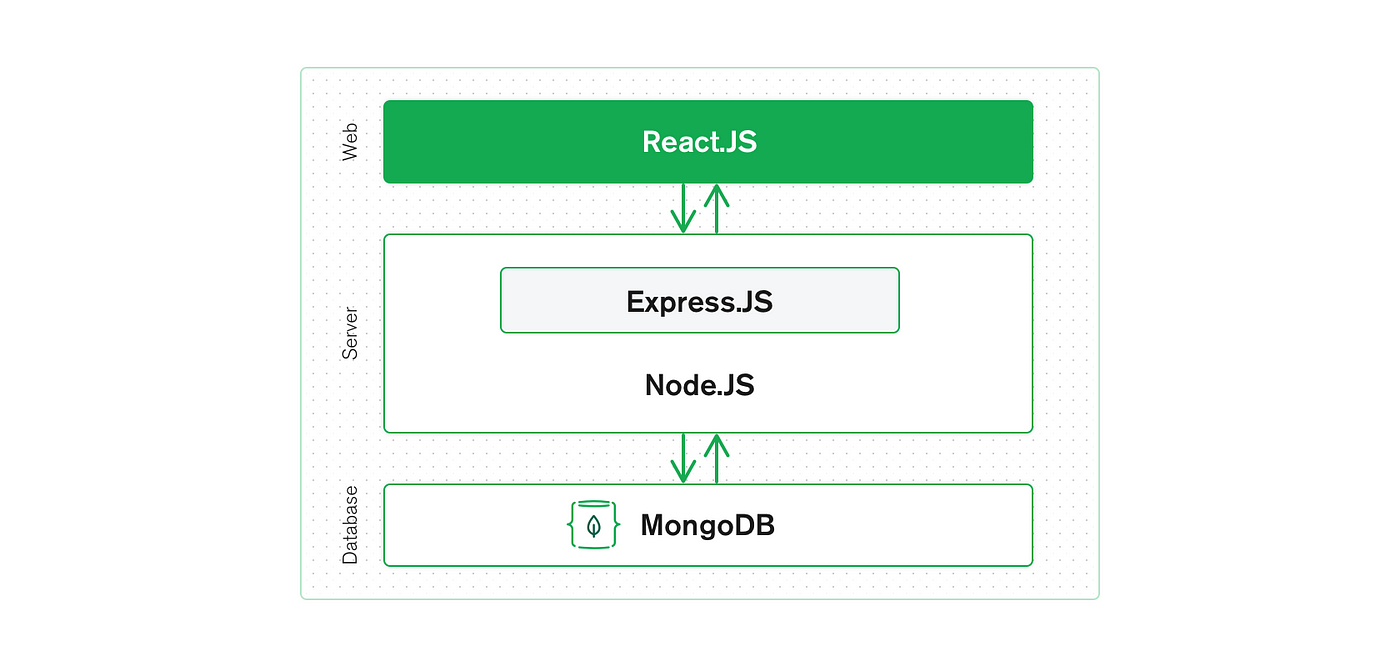
\includegraphics[width=12cm]{contents/chapter-2/mern_visualization.png}
	\caption{Diagram arsitektur \textit{stack} teknologi MERN \cite{s_what_2021}}
	\label{Fig:mern_visualization}
\end{figure}


Pada \textit{stack} teknologi MERN, MongoDB berperan sebagai \textit{database} untuk 
menyimpan data aplikasi web. MongoDB merupakan \textit{database} yang termasuk dalam kategori 
\textit{database} NoSQL yang bersifat \textit{document-oriented} dimana data disimpan dalam
bentuk kumpulan dokumen. Dokumen pada MongoDB disimpan dalam format BSON atau Binary JSON (\textit{JavaScript Object Notation})
yang terdiri dari pasangan \textit{key-value}. MongoDB bersifat \textit{schemaless} yang berarti
tidak memerlukan skema atau struktur yang tetap untuk setiap dokumen yang disimpan. 
Hal ini memudahkan \textit{developer} dalam mengembangkan aplikasi web karena tidak perlu
mengubah struktur \textit{database} jika terjadi perubahan pada aplikasi web. 
MongoDB memiliki fitur \textit{aggregation} yang memungkinkan \textit{developer} untuk
melakukan operasi agregasi seperti \textit{grouping, filtering, dan sorting} pada data yang
disimpan. MongoDB juga memiliki fitur \textit{indexing} yang memungkinkan \textit{developer} untuk
mengoptimalkan proses pencarian data pada \textit{database} \cite{boicea_mongodb_2012}. 
Dalam hal skalabilitas, MongoDB memiliki fitur \textit{sharding} yang memungkinkan \textit{developer} untuk 
membagi data menjadi beberapa bagian dan menyimpannya pada beberapa \textit{server} yang berbeda, 
sehingga dapat mengukur kapasitas aplikasi web yang dikembangkan\cite{kookarinrat_analysis_2015}

Pada \textit{stack} teknologi MERN, ExpressJS berperan sebagai \textit{framework} yang berjalan di atas NodeJS. 
ExpressJS Dicipptakan oleh TJ Holowaychuk pada tahun 2010\cite{vu_building_2020}. ExpressJS merupakan \textit{framework} yang 
bersifat \textit{unopinionated} yang berarti \textit{framework} ini tidak memiliki aturan atau struktur yang 
baku dalam mengembangkan aplikasi web\cite{lakshmi_website_2023}. Hal ini memungkinkan \textit{developer} untuk menentukan sendiri 
struktur aplikasi ExpressJS yang akan digunakan untuk mengembangkan aplikasi web. 
ExpressJS juga berbagai macam \textit{middleware} yang memungkinkan \textit{developer} 
untuk menambahkan fitur-fitur baru pada aplikasi web yang dikembangkan. ExpressJS juga memiliki 
\textit{routing} yang memungkinkan \textit{developer} untuk menentukan rute atau alamat URL yang akan 
diakses oleh pengguna. ExpressJS juga memiliki \textit{templating engine}, seperti Jade Engine, yang memungkinkan \textit{developer} 
untuk mengembangkan aplikasi web yang bersifat \textit{server-side rendering}\cite{jiang_architecture_2015}.

Pada \textit{stack} teknologi MERN, ReactJS berperan sebagai pustaka JavaScript untuk bagian \textit{User Interface} 
yang dikembangkan oleh Facebook. ReactJS menggunakan prinsip \textit{component-based} yang memungkinkan \textit{developer} 
untuk mengembangkan aplikasi web dengan membagi aplikasi web menjadi beberapa komponen yang dapat digunakan 
kembali. Hal ini memudahkan \textit{developer} dalam mengembangkan aplikasi web karena dapat mengurangi 
jumlah kode yang ditulis. Selain itu, penggunaan komponen juga dapat mengurangi waktu saat proses 
\textit{debugging} karena \textit{developer} hanya perlu mencari kesalahan pada komponen yang bermasalah.
ReactJS juga memiliki \textit{virtual DOM} yang memungkinkan \textit{developer}
untuk mengubah tampilan aplikasi web secara dinamis tanpa harus melakukan \textit{refresh} pada halaman web\cite{dinku_reactjs_2022}. 
ReactJS menggunakan state dan props untuk mengatur data yang akan ditampilkan pada aplikasi web. 
State merupakan data yang bersifat dinamis yang dapat berubah-ubah sesuai dengan kondisi aplikasi web. 
Props merupakan data yang bersifat statis yang tidak dapat berubah-ubah.

Pada \textit{stack} teknologi MERN, NodeJS berperan sebagai \textit{runtime environment} yang 
dikembangakn oleh Ryan Dahl pada tahun 2009. NodeJS memungkinkan kode JavaScript berjalan di luar \textit{browser} yaitu di sisi \textit{server}. 
NodeJS menggunakan \textit{event-driven} dan \textit{non-blocking I/O} yang memungkinkan NodeJS 
untuk menjalankan kode secara asinkronus. Hal ini memungkinkan NodeJS untuk menjalankan kode 
yang membutuhkan waktu yang lama tanpa harus menunggu kode tersebut selesai dijalankan. 
NodeJS juga memiliki \textit{package manager} yang bernama NPM (\textit{Node Package Manager}) 
yang memungkinkan \textit{developer} untuk mengunduh dan menginstal \textit{package} yang dibutuhkan 
untuk mengembangkan aplikasi web. \cite{rimal_developing_2019}

\subsection{Material UI}
Material UI adalah \textit{library} ReactJS yang berisi komponen-komponen yang dibuat berdasarkan Material Design 
yang dikembangkan oleh Google\cite{mannila_sales_2022}. Material UI menyediakan berbagai macam komponen React yang \textit{reusable}
yang dapat digunakan untuk mengembangkan aplikasi web. Material UI juga menyediakan dokumentasi yang lengkap 
mengenai komponen-komponen yang mereka sediakan, seperti \textit{button, icon, list, \emph{dan}dropdown},
serta bagaimana mengimplementasikannya pada aplikasi React yang sedang dikembangkan. 
Material UI juga memiliki \textit{theme} yang mempermudah \textit{developer} 
dalam mengkonfigurasi tema yang akan digunakan, seperti warna, ukuran, dan jenis font. 
Karena merupakan \textit{library} React, komponen-komponen tersebut memiliki \textit{style} 
penulisan kode yang sama seperti ReactJS, sehingga \textit{developer} yang sudah terbiasa 
menggunakan ReactJS tidak akan kesulitan dalam menggunakan Material UI.

\subsection{Json Web Token}
Menurut Website resminya, Json Web Token (JWT) adalah standar terbuka (RFC 7519) yang mendefinisikan cara untuk 
mengirimkan informasi secara aman antar pihak menggunakan objek JSON. Dalam pengembangan 
aplikasi web, JWT digunakan untuk mengautentikasi pengguna yang mengakses aplikasi. 
JWT terdiri dari tiga bagian, yaitu \textit{header, payload,} dan \textit{signature} seperti 
yang terlihat pada Gambar \ref{Fig:Struktur_JWT}.
\textit{Header} berisi informasi mengenai algoritma enkripsi yang digunakan untuk mengenkripsi \textit{payload}. 
\textit{Payload} berisi informasi pengguna yang akan digunakan untuk mengakses aplikasi web. 
\textit{Signature} berisi hasil enkripsi dari \textit{header} dan \textit{payload} menggunakan algoritma yang 
didefinisikan pada \textit{header}. Kemudian, ketiga bagian tersebut digabung dan di-\textit{encode} 
menjadi token string random yang sulit untuk dihapal.

\begin{figure}[h]
	\centering
	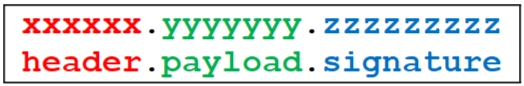
\includegraphics[width=6cm]{contents/chapter-2/struktur_jwt.jpg}
	\caption{Struktur JWT \cite{rahmatulloh_keamanan_2018}} 
	\label{Fig:Struktur_JWT}
\end{figure}

Salah satu kegunaan JWT pada suatu aplikasi web adalah untuk mengautentikasi \textit{user} yang mengakses aplikasi web. 
Pada saat \textit{user} melakukan \textit{login}, \textit{server} akan mengirimkan token JWT ke aplikasi web. 
Setelah itu, aplikasi web akan menyimpan token JWT pada \textit{local storage} atau \textit{session storage}. 
Token itulah yang harus disertakan setiap kali \textit{user} mengakses halaman web dan \textit{request resource \emph{dari} server}. 
Token tersebut akan dikirimkan ke \textit{server} untuk diverifikasi. Jika token tersebut valid, 
\textit{server} akan mengirimkan \textit{resource} yang diminta oleh \textit{user}. Gambar \ref{Fig:JWT_works} 
menunjukkan bagaimana JWT bekerja dalam mengautentikasi \textit{user} yang mengakses aplikasi web.

\begin{figure}[h]
	\centering
	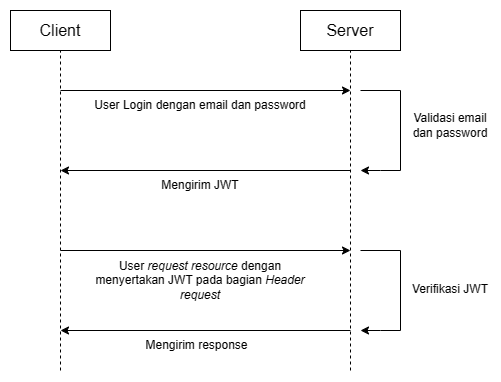
\includegraphics[width=9cm]{contents/chapter-2/jwt_works.png}
	\caption{Sequence diagram autentikasi JWT}
	\label{Fig:JWT_works}
\end{figure}


\subsection{Cloudinary}

Cloudinary merupakan suatu \textit{platform} manajemen media berbasis \textit{cloud} 
yang menyediakan solusi dalam penyimpanan, pengoptimalan, dan pengiriman file media 
seperti gambar, dokumen, video, dan audio\cite{ayuningtyas2017undangan}. Cloudinary 
memiliki berbagai fitur untuk menyederhanakan proses manajemen dan manipulasi 
aset media. Fitur-fitur tersebut dapat menjadi solusi bagi para 
\textit{software developer} dalam memanajemen file media pada aplikasi yang 
mereka kembangkan. Untuk memudahkan penggunanya, platform ini menyediakan 
dokumentasi yang lengkap mengenai berbagai layanan yang mereka tawarkan serta 
bagaimana cara menggunakannya. Cloudinary juga memiliki fleksibilitas yang 
baik dalam mendukung proses \textit{software development} karena API yang 
disediakan dapat terintegrasi dengan berbagai macam \textit{framework}, baik 
\textit{back-end, front-end, \emph{maupun} mobile} seperti yang terlihat pada
Gambar \ref{Fig:cloudinary_framework}, yang terdapat pada situs resminya\cite{cloudinary-website}.

\begin{figure}[h]
	\centering
	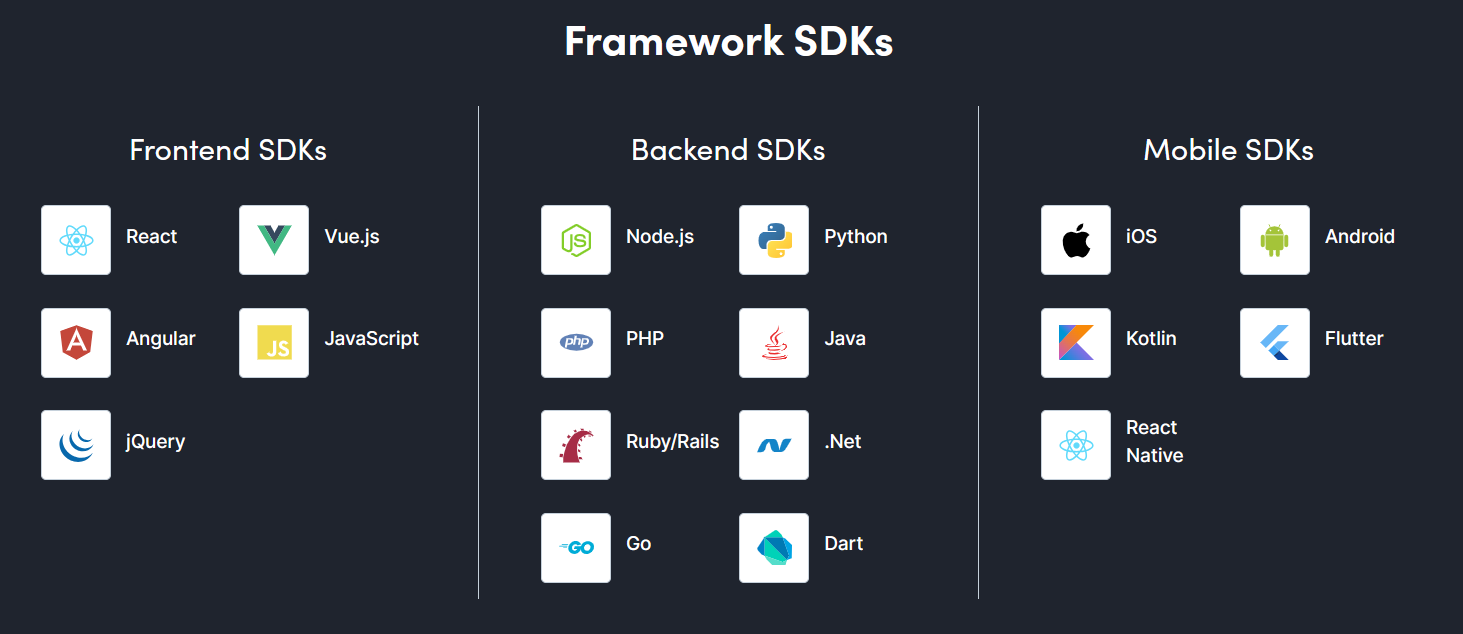
\includegraphics[width=12cm]{contents/chapter-2/cloudinary_framework.png}
	\caption{\textit{Framework} yang didukung oleh Cloudinary \cite{cloudinary-website}}
	\label{Fig:cloudinary_framework}
\end{figure}

% \subsection{\textit{Entity Relationship Diagram}(ERD)}


% \subsection{\textit{Use Case Diagram}}
% \textit{Use case diagram} adalah diagram yang menggambarkan interaksi antara \textit{user} dengan sistem yang dibuat. 
% \textit{Use case diagram} terdiri dari \textit{actor, use case,} dan \textit{relationship}. 
% \textit{Actor} adalah entitas yang berinteraksi dengan sistem. \textit{Use case} adalah 
% fungsi-fungsi yang dapat dilakukan oleh \textit{actor}. \textit{Relationship} adalah 
% hubungan antara \textit{actor} dan \textit{use case}. Gambar \ref{Fig:Use_Case_Diagram}
% menunjukkan \textit{use case diagram} dari aplikasi yang dibuat. 
\subsection{Metode Pengembangan \textit{Software}}
Dalam mengembangkan suatu aplikasi atau \textit{software}, terdapat beberapa metode yang dapat digunakan. 
Metode tersebut dapat digunakan untuk mengatur proses pengembangan \textit{software} agar dapat 
dilakukan dengan lebih terstruktur dan terarah. Dalam dunia \textit{software development}, metode 
pengembangan \textit{software} dikenal dengan sebutan \textit{software development life cycle} (SDLC). 
SDLC adalah suatu proses yang terstruktur untuk mengembangkan \textit{software} yang terdiri dari 
beberapa tahapan. Tahapan-tahapan tersebut dapat disesuaikan dengan kebutuhan dan karakteristik 
dari \textit{software} yang akan dikembangkan. Pada bagian ini, akan dijelaskan mengenai 
dua metode SDLC yang dapat digunakan dalam mengembangkan \textit{software} yaitu metode 
\textit{waterfall} dan metode \textit{agile}.

\subsubsection{Metode SDLC Waterfall}
Metode \textit{waterfall} adalah metode SDLC yang paling sederhana. Metode \textit{waterfall} 
pertama kali diperkenalkan oleh Winston W. Royce pada tahun 1970\cite{bassil_simulation_2012}. Metode ini terdiri dari 
beberapa tahapan yang harus dilakukan secara berurutan dan sekuensial. Tahapan-tahapan tersebut adalah 
\textit{requirement analysis, system design, implementation, testing,} dan \textit{maintenance}. 
Gambar \ref{Fig:Waterfall_step} menunjukkan tahapan-tahapan dalam metode \textit{waterfall}. 
Pada Gambar \ref{Fig:Waterfall_step}, prosesnya mengalir dari satu tahapan ke tahapan lain 
seperti halnya air terjun yang mengalir turun secara berurutan.

\begin{figure}[h]
	\centering
	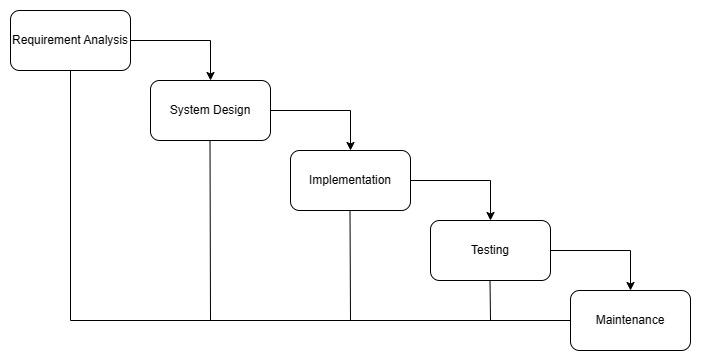
\includegraphics[width=9cm]{contents/chapter-2/waterfall_fig.png}
	\caption{Tahapan dalam metode SDLC \textit{waterfall}}
	\label{Fig:Waterfall_step}
\end{figure}

Metode Waterfall memiliki kelebihan dan kekurangan. 
Metode Waterfall merupakan metode yang mudah dipahami dan digunakan, terutama oleh \textit{developer} 
pemula. 
Metode Waterfall cocok digunakan untuk mengembangkan \textit{software} yang memiliki 
\textit{requirement} yang jelas dan cenderung tidak akan mengalami perubahan \textit{requirement} 
di tengah proses pengembangan. Metode ini juga cocok digunakan pada \textit{project} kecil 
yang memiliki risiko yang rendah. Metode ini tidak cocok digunakan 
untuk mengembangkan \textit{software} yang memiliki risiko yang tinggi karena 
metode ini tidak memiliki mekanisme untuk mengatasi perubahan \textit{requirement} 
di tengah proses pengembangan. Metode ini juga tidak cocok digunakan untuk 
mengembangkan \textit{software} yang memiliki \textit{requirement} yang tidak jelas. 
Hal ini dikarenakan metode ini tidak memiliki tahapan untuk melakukan analisis 
\textit{requirement} yang mendalam. 

\subsubsection{Metode SDLC Agile}
Metode \textit{agile} adalah metode SDLC yang paling fleksibel. Metode ini terdiri dari 
beberapa tahapan yang dapat dilakukan secara berulang-ulang atau bersifat \textit{iterative}. 
Terjadinya pengulangan tahapan biasanya disebabkan oleh sistem yang dikembangkan memiliki 
\textit{requirement} yang belum jelas atau dapat berubah sewaktu-waktu. Metode Agile 
berfokus pada adaptabilitas, fleksibilitas, dan kemampuan untuk bergerak dengan cepat, sesuai dengan 
namanya, yaitu \textit{agile} yang berarti lincah. Gambar \ref{Fig:Agile_step} merupakan 
lustrasi bagaimana metode Agile pada \textit{software development life cycle} (SDLC).

\begin{figure}[h]
	\centering
	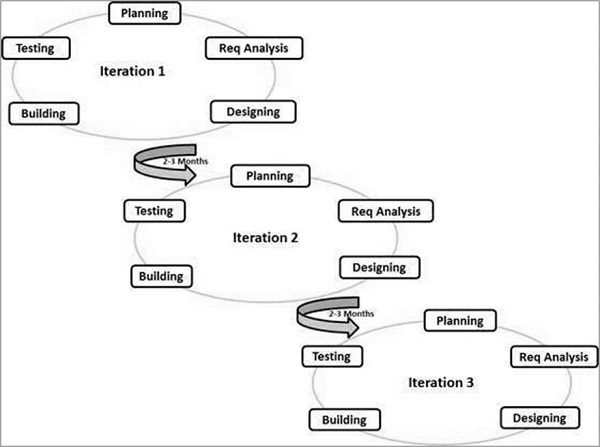
\includegraphics[width=9cm]{contents/chapter-2/sdlc_agile_model.jpg}
	\caption{Tahapan dalam metode SDLC \textit{Agile}\cite{noauthor_sdlc_nodate}}
	\label{Fig:Agile_step}
\end{figure}

Gambar \ref{Fig:Agile} menunjukkan tahapan-tahapan dalam metode \textit{agile}. 
Metode ini cocok digunakan untuk mengembangkan \textit{software} yang memiliki 
\textit{requirement} yang tidak jelas dan dapat berubah sewaktu-waktu. Metode ini 
juga cocok digunakan untuk mengembangkan \textit{software} yang memiliki risiko yang 
tinggi. Hal ini dikarenakan metode ini memiliki mekanisme untuk mengatasi perubahan 
\textit{requirement} di tengah proses pengembangan. Metode ini juga cocok digunakan 
untuk mengembangkan \textit{software} yang memiliki \textit{requirement} yang jelas. 
Metode ini tidak cocok digunakan untuk mengembangkan \textit{software} yang memiliki 
risiko yang rendah karena metode ini memiliki tahapan yang berulang-ulang dan 
membutuhkan waktu yang lebih lama dibandingkan dengan metode \textit{waterfall}. 
Metode ini juga tidak cocok digunakan untuk mengembangkan \textit{software} yang 
memiliki \textit{requirement} yang tidak jelas. Hal ini dikarenakan metode ini tidak 


\section{Analisis Perbandingan Metode}

% Di dalam tinjauan pustaka hasil akhirnya adalah analisis secara kualitatif atau pun secara kuantitatif kelebihan dan kekurangan metode jika dikaitkan dengan masalah, batasan-batasan masalah dan solusi yang dinginkan. Analisis kuantitatif tidak wajib teapi mempunyai nilai tambah di dalam tugas akhir saudara. Bagian ini menjelaskan kenapa metode tersebut dipilih dan uraikan dengan lebih jelas metode pelaksanaan tugas akhir yang ingin Anda lakukan. 

Pada bagian ini, akan dilakukan perbandingan metode-metode untuk mengembangkan aplikasi web, 
yang akan digunakan untuk mengembangkan sistem informasi penelitian dan pengabdian kepada 
masyarakat. Pemilihan metode didasarkan pada kompleksitas dan ukuran aplikasi, fleksibilitas 
, waktu, jumlah anggota tim, dan sebagainya. 

Seperti yang telah disebutkan pada bagian 2.2.7 mengenai metode pengembangan \textit{software}, 
metode \textit{waterfall} dan metode \textit{agile} merupakan dua dari beberapa metode 
pengembangan \textit{software} yang dapat digunakan. 

Keduanya memiliki kelebihan dan 
kekurangan masing-masing dan cenderung saling bertolak belakang. Metode \textit{waterfall} 
memiliki tahapan yang berurutan dan sekuensial, sehingga cocok digunakan untuk mengembangkan 
\textit{software} yang memiliki \textit{requirement} yang jelas dan cenderung tidak akan 
mengalami perubahan \textit{requirement} di tengah proses pengembangan. Metode \textit{agile} 
memiliki tahapan yang dapat dilakukan secara berulang-ulang atau bersifat \textit{iterative}, 
sehingga cocok digunakan untuk mengembangkan \textit{software} yang memiliki \textit{requirement} 
yang tidak jelas dan dapat berubah sewaktu-waktu. 
\chapter{Metode Penelitian}

Bab ini menjelaskan metode atau cara yang digunakan dalam penelitian ini untuk 
mencapai maksud dan tujuan seperti yang tertulis dalam sub-bab 1.3 [jika diinginkan, kalian dapat menuliskan Kembali tujuan penelitian yang ingin dicapai di sini].

\section{Alat dan Bahan Tugas akhir}

\subsection{Alat Tugas akhir}

Alat-alat yang digunakan pada tugas akhir ini berupa perangkat keras maupun perangkat lunak dengan spesifikasi sebagai berikut:

\begin{enumerate}
	\item \textit{Notebook} ASUS Vivobook dengan spesifikasi sistem operasi Windows 11, \textit{processor} Intel Core i5-1235U, 16GB RAM DDR4, Intel Iris Xe, SSD 500GB.
	\item \textit{Browser} Microsoft Edge untuk menjalankan aplikasi \textit{front-end}.
	\item \textit{Text Editor} Visual Studio Code untuk \textit{coding} aplikasi \textit{front-end} dan \textit{back-end}.
	\item MongoDB Atlas \textit{dashboard} untuk mengelola \textit{database} sistem informasi.
	\item Cloudinary \textit{Digital Asset Management} untuk mengelola \textit{cloud storage} dengan data yang berbentuk media seperti gambar dan  \textit{document}
	\item Aplikasi diagrams.net untuk merancang \textit{flowchart, Entity Relationship Table, dan Use Case Diagram}.
	\item ReactJs versi 18.2.0 untuk \textit{front-end} aplikasi.
	\item NodeJs versi 18.15.0 untuk \textit{runtime environment} aplikasi \textit{back-end}.
	\item ExpressJs versi 4.18.2 untuk \textit{framework} aplikasi \textit{back-end}.
	\item \textit{Node Package Manager} (NPM) versi 9.5.0 untuk mengelola \textit{dependencies} aplikasi.
	\item Json Web Token versi 9.0.0 untuk proses \textit{authentication} dan \textit{authorization}.
	\item Cloudinary Node SDK versi 1.35.0 untuk menghubungkan aplikasi dengan \textit{cloud storage} Cloudinary.
	\item Mongoose versi 7.0.11 untuk menghubungkan aplikasi dengan \textit{database} MongoDB.
	\item Material UI versi 5.13.0 untuk mengelola komponen \textit{User Interface} pada aplikasi.
	\item Postman untuk melakukan \textit{testing} API.
\end{enumerate}
\subsection{Bahan Tugas akhir}

Bahan yang digunakan pada tugas akhir ini yaitu berupa data yang diperoleh dari Dosen 
Pembimbing yaitu berupa \textit{requirement} sistem informasi yang akan dikembangkan. 
Detail mengenai bagaimana \textit{requirement} tersebut didapatkan akan dijelaskan pada Bab 3.

% Bahan tugas akhir adalah segala sesuatu yang bersifat fisik atau digital yang digunakan untuk kebutuhan tugas akhir. Bahan tugas akhir dapat berupa:

% \begin{enumerate}
% 	\item Bahan habis pakai. Bahan yang digunakan untuk tugas akhir. Sebagai contoh 
% 	mungkin dibutuhkan kertas transparansi, baterai, atau yang lain 
% 	\item Bahan yang berupa data atau informasi yang menjadi dataset tugas akhir. Dataset tugas akhir dapat berupa:
% \end{enumerate}
% \begin{itemize}
% 	\item Dataset pihak lain yang diperoleh dengan izin atau dalam lisensi yang diizinkan untuk digunakan secara langsung 
% 	\item Dataset pihak pertama yang disusun sendiri melalui quisioner, observasi, atau interview 
% 	\item Dokumen panduan yang mengacu pada standar, hasil tugas akhir, atau artikel yang disitasi dan digunakan.
% \end{itemize}


\section{Metode yang Digunakan}

Bagian ini membahas metode atau cara yang akan digunakan dalam penelitian, tahapan 
penerapan metode, dan desain penelitian (misalnya apakah penelitian akan menggunakan 
eksperimen di Laboratorium atau di lapangan, misalkan saja penelitian biomedis atau 
penelitian alat ukur hama yang dapat dilakukan di laboratorium ataupun di lapangan, atau menggunakan metode survei (misalnya untuk teknologi Informasi), studi kasus, atau analisis dengan perangkat lunak (ETAP, LTSpice, dst), atau \textit{prototyping} (pembuatan perangkat keras).

Bagian ini juga membahas bagaimana data [akan] dianalisis, apakah dengan membandingkan keluaran beberapa alat ukur, membandingkan dengan standar atau bagaimana.

\section{Alur Tugas Akhir}

Menguraikan prosedur yang akan digunakan dan jadwal atau alur penyelesaian setiap 
tahap. Alur penelian ini dapat disajikan dalam bentuk diagram. Diagram dapat disusun dengan aturan yang baik semisal menggunakan \textit{flowchart}. Aturan dan tutorial pembuatan \textit{flowchart} dapat dilihat di \textcolor{blue}{http://ugm.id/flowcharttutorial}. Setelah menggambarkannya, penulis wajib menjelaskan langkah-langkah setiap alur tugas akhir dalam sub bab tersendiri sesuai dengan kebutuhan.

% \section{Etika, Masalah, dan Keterbatasan Penelitian (Opsional))}

% Bagian ini membahas pertimbangan etis penelitian dan [potensi] masalah serta
% keterbatasannya. Jika menyangkut penelitian dengan makhluk hidup, maka dibutuhkan adanya \textit{ethical clearance}, di bagian ini hal itu akan dibahas. Demikian juga tentang keterbatasan ataupun masalah yang akan timbul.

\chapter{Hasil dan Pembahasan}

\section{Pembahasan Hasil 1 (Ubah Judul Sesuai dengan Hal yang Hendak dibahas)}

Poin pertama adalah membahas tujuan penelitian pertama. 
Dapat ditambahkan beberapa sub bab jika diperlukan.

\section{Pembahasan Hasil 2 (Ubah Judul Sesuai dengan Hal yang Hendak dibahas)}

Poin kedua adalah membahas tujuan penelitian kedua. Dapat ditambahkan beberapa 
sub bab jika diperlukan. Dapat juga diteruskan ke Sub Bab Pembahasan hasil 3 dan 
seterusnya, jika ada tiga atau lebih tujuan penelitian.

\section{Perbandingan Hasil Penelitian dengan Hasil Terdahulu}

Pembahasan penutup dapat menjelaskan mengenai kelebihan hasil pengembangan / 
penelitian dan kekurangan dibandingkan dengan skripsi atau penelitian terdahulu atau
perbandingan terhadap produk lain yang ada di pasaran. Penulis dapat menggunakan tabel untuk membandingkan secara gamblang dan menjelaskannya.
\chapter{Tambahan (Opsional)}

Anda boleh menambahkan Bab jika diperlukan. Jumlah Bab tidak harus sesuai dengan \textit{template}. 

\chapter{Kesimpulan dan Saran}

\section{Kesimpulan}

Kesimpulan dapat diawali dengan apa yang dilakukan dengan tugas akhir ini lalu 
dilanjutkan dengan poin-poin yang menjawab tujuan penelitian, apakah tujuan sudah tercapai atau belum, tentunya berdasarkan data ataupun hasil dari Bab pembahasan sebelumnya. Dalam beberapa hal, kesimpulan dapat juga berisi tentang temuan/\textit{findings} yang Anda dapatkan setelah melakukan pengamatan dan atau analisis terhadap hasil penelitian. 

\section{Saran}

Saran berisi hal-hal yang bisa dilanjutkan dari penelitian atau skripsi ini, yang belum dilakukan karena batasan permasalahan. Saran bukan berisi saran kepada sistem atau pengguna, tetapi saran diberikan kepada aspek penelitian yang dapat dikembangkan dan ditambahkan di penelitian atau skripsi selanjutnya.


%======================================

%======================================
%  References
%======================================
\thereferences
% You can change 
%    the filename and location of the files inputted
\bibliography{references}

%Hapus bagian di bawah setelah tidak diperlukan
\begin{center}
	\textcolor{red}{
	Catatan: Daftar pustaka adalah apa yang dirujuk atau disitasi, bukan apa yang telah dibaca, jika tidak ada dalam sitasi maka tidak perlu dituliskan dalam daftar pustaka.}
\end{center}

%======================================

%======================================
%  Appendix
%======================================
% You can change 
%    the filename and location of the files inputted
%    use \chapterappendix for the first page of the appendix
%    use \chapterappendixadd for the next page

\appendix


\chapterappendix{contents/appendix/appendix-isi-lampiran}
\chapterappendixadd{contents/appendix/appendix-latex}
\chapterappendixadd{contents/appendix/appendix-penulisan-referensi}
\chapterappendixadd{contents/appendix/appendix-code}




%======================================

\end{document}